\documentclass[12pt,compress,ngerman,utf8,t]{beamer}
\usepackage{etex}
\usepackage[ngerman]{babel}
\usepackage{graphicx}
\usepackage[export]{adjustbox}
\usepackage{multicol}


\usetheme[numbering=fraction, progressbar=frametitle]{metropolis}


\date{\today}
\institute{University of Freiburg}
\titlegraphic{\hspace{9cm} 
\includegraphics[height=2cm]{template/Logo-Uni-Freiburg.png}}
\graphicspath{ {./template/} {./strategy/} }

\title{Strategie}
\author{Felix Karg}
\subject{Mathecamp}


\AtBeginSection[]
{
    \begin{frame}{Inhalt}
        \begin{multicols}{2}
            \small
            \tableofcontents[currentsection]
        \end{multicols}
        \clearpage
    \end{frame}
}

\AtBeginSubsection[]
{
    \small
    \begin{frame}{Inhalt}
        \begin{multicols}{2}
            \small
            \tableofcontents[currentsection,currentsubsection]
        \end{multicols}
        \clearpage
    \end{frame}
}

% \vspace{0.1cm}

\begin{document}

\maketitle

% multicols from:
% https://tex.stackexchange.com/questions/24343/splitting-toc-into-two-columns-on-single-frame-in-beamer

\begin{frame}{Inhalt}
    \small
    \begin{multicols}{2}
        \small
        \tableofcontents[hidesubsections]
    \end{multicols}
    \clearpage
\end{frame}



%%%%%%%%%%%%%%%%%%%%%%%%%%%%%%%%%%%%%%%%%%%%%%%%%%SECTION%%%%%%%%%%%%%%%%%%%%%%%%%%%%%%%%%%%%%%%%%%%%%%%%%%
\section{Hindernisse Überkommen}
%%%%%%%%%%%%%%%%%%%%%%%%%%%%%%%%%%%%%%%%%%%%%%%%%%SECTION%%%%%%%%%%%%%%%%%%%%%%%%%%%%%%%%%%%%%%%%%%%%%%%%%%

\begin{frame}[c]{Warum ist Strategie überhaupt wichtig?}
    Mehrere Gründe, vor allem: \\
    \pause
    \begin{itemize}
        \item Das Leben besteht aus lauter Problem
            \pause
        \item Strategisch zu Denken hilft einem Sinnvolle Entscheidungen zu treffen
            \pause
        \item Oder: Mathematische Probleme Strategisch zu betracheten
            \pause
        \item Das 'Spiel Gewinnen'
            \pause
        \item Einen Vorteil haben, der jedem Zugänglich ist
            \pause
        \item Allgemein: Problemstellungen mit Neuen Werkzeugen Bezwingen
    \end{itemize}
\end{frame}


%%%%%%%%%%%%%%%%%%%%%%%%%%%%%%%%%%%%%%%%%%%%%%%%%%SECTION%%%%%%%%%%%%%%%%%%%%%%%%%%%%%%%%%%%%%%%%%%%%%%%%%%
\section{Disclaimer}
%%%%%%%%%%%%%%%%%%%%%%%%%%%%%%%%%%%%%%%%%%%%%%%%%%SECTION%%%%%%%%%%%%%%%%%%%%%%%%%%%%%%%%%%%%%%%%%%%%%%%%%%
\begin{frame}[c]{Disclaimer}
    Ein paar beispiele kommen aus der Welt der Wirtschaft. \\ \pause

    \vfill

    Das heißt aber noch lange nicht, dass sich Strategie nur dort anwenden lässt.
\end{frame}



%%%%%%%%%%%%%%%%%%%%%%%%%%%%%%%%%%%%%%%%%%%%%%%%%%SECTION%%%%%%%%%%%%%%%%%%%%%%%%%%%%%%%%%%%%%%%%%%%%%%%%%%
\section{Mächtigkeit guter Strategie}
%%%%%%%%%%%%%%%%%%%%%%%%%%%%%%%%%%%%%%%%%%%%%%%%%%SECTION%%%%%%%%%%%%%%%%%%%%%%%%%%%%%%%%%%%%%%%%%%%%%%%%%%

\subsection{Napoleon gegen die Briten}

\begin{frame}[c, fragile]{Schlacht von Trafalgar I}
    Napoleon (Villeneuve):
    \begin{itemize}
        \item Frankreich + Spanien
        \item<2-> \verb!   18    +   15   ! Linienschiffe
        \item<2-> \verb!   08    +   00   ! Andere
        \item<3-> Summe: 41 Schiffe
    \end{itemize}

    Lord Nelson:
    \begin{itemize}
        \item England
        \item<2-> 27 Linienschiffe
        \item<2-> 06 Andere
        \item<3-> Summe: 33 Schiffe
    \end{itemize}
    \pause
    \pause
    \pause

    Wer Gewinnt also?
\end{frame}

\begin{frame}{Schlacht von Trafalgar II}
    Aber wie? \\
    \pause
    Traditionelle See-Schlachten: Linienkämpfe \\
    \pause
    Nelsons Plan: \\
    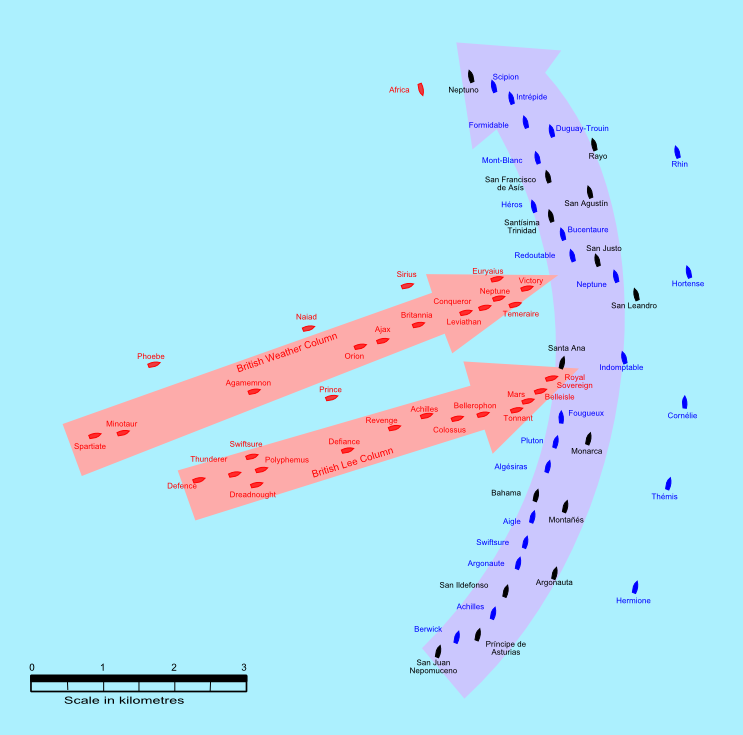
\includegraphics[height=6cm]{strategy/Trafalgar-1200hr.jpg}
\end{frame}

\begin{frame}{Schlacht von Trafalgar III}
    \begin{multicols}{2}
        Verluste für Villeneuve (Napoleon) \\
        Frankreich:
        \begin{itemize}
            \item<2-> 10 Schiffe
            \item<2-> 1 Schiff Zerstört
            \item<3-> 2'218 Tote
            \item<3-> 1'155 Verletzte
            \item<4-> ~4'000 Gefangene
        \end{itemize}
        Spanien:
        \begin{itemize}
            \item<2-> 11 Schiffe
            \item<3-> 1'025 Tote
            \item<3-> 1'383 Verletzte
            \item<4-> ~4'000 Gefangene
        \end{itemize}
        \visible<5> {Summe: 22 Schiffe + 13'781 Außer Gefecht}


        Verluste für die Briten
        \begin{itemize}
            \item<2-> Kein einziges Schiff
            \item<3-> 458 Tote
            \item<3-> 1'208 Verletzte
            \item<5-> Insgesamt: 1'666 Außer Gefecht
        \end{itemize}

        \pause
        \pause
        \pause
        \pause

    \end{multicols}

\end{frame}



\subsection{Steve Jobs Rettet Apple}

\begin{frame}{Steve Jobs Rettet Apple I}
    September 1997. \\
    Apple ist 2 Monate entfernt von Insolvenz. \\
    \pause
    Angebot: \\
    \begin{itemize}
        \item 15 verschiedene Desktop-Rechner
        \item Unglaublich viele Laptops (+ ähnliches)
        \item Mehrere Drucker etc.
        \item 6 Apple-Stores
    \end{itemize}
    \pause

    Was hat er also getan?

\end{frame}

\begin{frame}{Steve Jobs Rettet Apple II}
    Er hat das Offensichtliche Getan\pause,
    danach gab es:
    \begin{itemize}
        \item 1 Desktop-Rechner
        \item 1 Laptop
        \item Keine Drucker oder ähnliches
        \item 1 Apple Store
        \item viel weniger Entwickler !!
        \item Produktion in Taiwan
        \item Inventarverkleinerung (80\%)
        \item Neuer Web-Store
    \end{itemize}
    \pause
    Das erschreckende ist, wie viel davon Wirtschafts-101 ist,
    und dennoch Unerwartet war. \\
    \pause
    Außerdem Bat er Bill Gates um 150Millionen
\end{frame}

\begin{frame}[c]{Steve Jobs Rettet Apple III}
    \Large
    Was war sein Plan für die Zukunft? \\
    \pause

    Steve Jobs: ``Ich warte auf das nächste große Ding.''

\end{frame}

\subsection{Strategie ist Unerwartet}




%%%%%%%%%%%%%%%%%%%%%%%%%%%%%%%%%%%%%%%%%%%%%%%%%%SECTION%%%%%%%%%%%%%%%%%%%%%%%%%%%%%%%%%%%%%%%%%%%%%%%%%%
\section{Nicht-Strategie}
%%%%%%%%%%%%%%%%%%%%%%%%%%%%%%%%%%%%%%%%%%%%%%%%%%SECTION%%%%%%%%%%%%%%%%%%%%%%%%%%%%%%%%%%%%%%%%%%%%%%%%%%

\subsection{Beispiele für Nicht-Strategie}

\begin{frame}[c]{Beispiele für Nicht-Strategie}
    Zielsetzung: z.B.: \pause
    \begin{itemize}
        \item Ich werde Eine Gute Note schreiben! \pause
        \item Wir werden Dieses Jahr Erfolgreicher als jeher! \pause
        \item Wir werden den Gegner vernichtend Schlagen! \pause
    \end{itemize}

    Oder auch:
    \begin{itemize}
        \item Nicht aufhören, bis man sein Ziel erreicht \pause
        \item Ich möchte eine Gute Note schreiben. Daher esse ich Kuchen.
    \end{itemize}
\end{frame}

\begin{frame}[c]{Nicht-Strategie}
    \large
    \begin{itemize}
        \item Flauschige Ziele \pause
        \item Vision \pause
        \item Die Herausforderung verfehlen \pause
        \item Inkonsistente Ziele / Aktionen \pause
    \end{itemize}
\end{frame}


\begin{frame}{Flauschige Ziele}
    
\end{frame}


\begin{frame}{Strategie Falsch interpretieren}
    
\end{frame}


\begin{frame}{Die Herausforderung verfehlen}
    Beispiel: Ich möchte eine Gute Note schreiben. Daher esse ich Kuchen.
\end{frame}


\begin{frame}{Inkonsistente Ziele / Aktionen}
    
\end{frame}


\subsection{Warum wird so vieles für Strategie gehalten?}


%%%%%%%%%%%%%%%%%%%%%%%%%%%%%%%%%%%%%%%%%%%%%%%%%%SECTION%%%%%%%%%%%%%%%%%%%%%%%%%%%%%%%%%%%%%%%%%%%%%%%%%%
\section{Analyse}
%%%%%%%%%%%%%%%%%%%%%%%%%%%%%%%%%%%%%%%%%%%%%%%%%%SECTION%%%%%%%%%%%%%%%%%%%%%%%%%%%%%%%%%%%%%%%%%%%%%%%%%%
\begin{frame}{Analyse I - Finden versteckter Stärken}
    % Mehrere Optionen:
    %   Wal-Mart (?)
    %   David & Goliath (?) (Melly fragen!)
    %   Dosen-Abfüll-Dings (?)
\end{frame}



%%%%%%%%%%%%%%%%%%%%%%%%%%%%%%%%%%%%%%%%%%%%%%%%%%SECTION%%%%%%%%%%%%%%%%%%%%%%%%%%%%%%%%%%%%%%%%%%%%%%%%%%
\section{Echte Strategie}
%%%%%%%%%%%%%%%%%%%%%%%%%%%%%%%%%%%%%%%%%%%%%%%%%%SECTION%%%%%%%%%%%%%%%%%%%%%%%%%%%%%%%%%%%%%%%%%%%%%%%%%%
\subsection{Kernelemente echter Strategie}
\subsection{Sich einen Vorteil verschaffen}
\subsection{Fokus}
\subsection{Design}
\subsection{Einen Vorteil verwenden}



%%%%%%%%%%%%%%%%%%%%%%%%%%%%%%%%%%%%%%%%%%%%%%%%%%SECTION%%%%%%%%%%%%%%%%%%%%%%%%%%%%%%%%%%%%%%%%%%%%%%%%%%
\section{Beispiele für Gute Strategie}
%%%%%%%%%%%%%%%%%%%%%%%%%%%%%%%%%%%%%%%%%%%%%%%%%%SECTION%%%%%%%%%%%%%%%%%%%%%%%%%%%%%%%%%%%%%%%%%%%%%%%%%%

\begin{frame}{Reminder: Gute Strategie}
    Gute Strategie besteht aus:
    \begin{itemize}
        \item Einer Leit-Idee
        \item Einem Ziel
        \item Einem Plan an Kohärenten Aktionen, um zu diesem Ziel zu gelangen
    \end{itemize}
\end{frame}

\begin{frame}[c]{Gute Strategie: Beispiel Intel}
    Intel hat einiges Richtig gemacht:
    \begin{itemize}
        \item War ursprünglich Arbeitsspeicher-Hersteller \pause
        \item Radikaler Umschwung z
    \end{itemize}
\end{frame}



\begin{frame}[c]{Gute Strategie: Beispiel SpaceX}
    Wie sah die Raumfahrt-Industrie vor SpaceX aus? \pause
    

    Es gab:
    \begin{itemize}
        \item die ULA (United Launch Alliance)
        \item Arianespace (ESA-basiert)
        \item Das Russische Kommerzielle Programm
        \item (Das Chinesische und Japanische Raumfahrt-Programm)
    \end{itemize}

\end{frame}



\begin{frame}[c]{Raketen}

    \begin{tabular}{l|l|l|l|l}
        Wer &   Rakete         &   zum LEO &  zum GTO  &  Kosten         \\ \hline
        ULA & Delta IV (Heavy) & 22'560 Kg & 13'400 Kg & 400 Mio \$      \\ \hline
        ULA & Atlas V          & 18'510 Kg &  8'900 Kg & 150 Mio \$      \\ \hline
        ESA & Ariane 5         & 20'000 Kg & 10'500 Kg & 220 Mio \$      \\ \hline
        ESA & Soyuz II         &  8'200 Kg &  3'250 Kg & 60 Mio  \$      \\ \hline
        ILS & Proton-M         & 23'000 Kg &  6'920 Kg & 150 Mio \$      \\
    \end{tabular}


    \footnotesize
    Disclaimer: es ist sehr Schwer Korrekte Preis-Angaben zu finden, da diese meist nicht Öffentlich sind.
    Auch die Traglasten sind nicht exakt Angebbar, da ständig irgendwelche Verbesserungen (zumindest in letzter Zeit)
    gemacht werden.

\end{frame}


\begin{frame}[c]{SpaceX}

    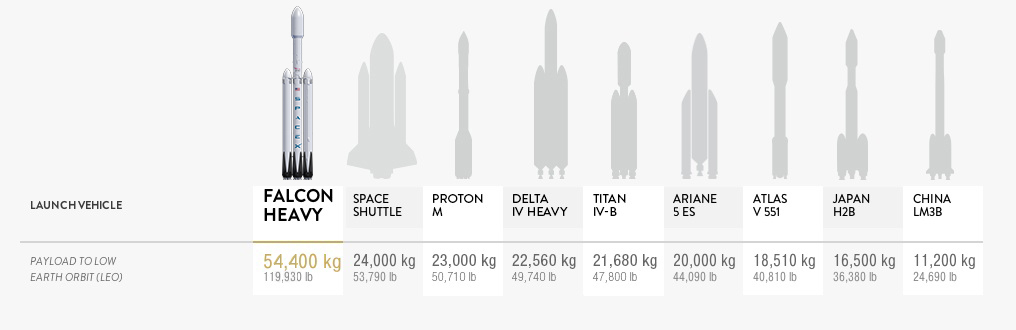
\includegraphics[height=3cm]{strategy/comparison.jpg} \\

    \begin{tabular}{l|l|l|l|l}
        Rakete       & zum LEO   & zum GTO   & Traglast zum Mars & Kosten \\ \hline
        Falcon 9     & 22'000 Kg &  8'300 Kg &  4'200 Kg         & 60Mio  \\ \hline
        Falcon Heavy & 54'400 Kg & 22'200 Kg & 13'400 Kg         & 90Mio  \\
    \end{tabular}


    \footnotesize
    Unter der Annahme, dass die Booster / Erste Stufe nicht wiederverwendet wird.
    Andernfalls sind ca. 30\% der Traglast abzuziehen

\end{frame}


%%%%%%%%%%%%%%%%%%%%%%%%%%%%%%%%%%%%%%%%%%%%%%%%%%SECTION%%%%%%%%%%%%%%%%%%%%%%%%%%%%%%%%%%%%%%%%%%%%%%%%%%
\section{Quellen}
%%%%%%%%%%%%%%%%%%%%%%%%%%%%%%%%%%%%%%%%%%%%%%%%%%SECTION%%%%%%%%%%%%%%%%%%%%%%%%%%%%%%%%%%%%%%%%%%%%%%%%%%
\begin{frame}[c,fragile,allowframebreaks]{Quellen}
    Die Folien sind zu finden unter: \\
    \url{https://github.com/blueburningcoder/things-to-talk-about/tree/master/strategy}


    Das Buch, aus dem ich den Vortrag gebastelt hab:

    \begin{thebibliography}{10}
    \beamertemplatebookbibitems
    \bibitem{Richard Rumelt}
        Richard Rumelt
        \newblock {\em Good Strategy / Bad Strategy}.
        \newblock The Difference and Why It Matters \\
                  ISBN: 978-1-78125-154-6
    \beamertemplatearticlebibitems
    \bibitem{Wikipedia}
        Wikipedia
            \newblock {\em Battle of Trafalgar}
            \newblock \url{https://en.wikipedia.org/wiki/Battle\_of\_Trafalgar}
    \bibitem{Wikipedia}
        Wikipedia
            \newblock {\em SpaceX}
            \newblock \url{Dunno}
    \bibitem{Wihipedia}
        Wikipedia
            \newblock {\em Proton-M}
            \newblock \url{https://en.wikipedia.org/wiki/Proton-M}
    \bibitem{Wikipedia}
        Wikipedia
            \newblock {\em Ariane 5}
            \newblock \url{https://en.wikipedia.org/wiki/Ariane\_5}
    \bibitem{Wikipedia}
        Wikipedia
            \newblock {\em Delta IV Heavy}
            \newblock \url{https://en.wikipedia.org/wiki/Delta\_IV}
    \end{thebibliography}
    % required the allowframebreaks for longer lists


\end{frame}


\end{document}
